
\chapter{The SECD Machine}

There are many different types of model used to analyse programs and
programming languages. These include models of source code, e.g. flow-graphs,
models of type systems, models of pre and post conditions, petri-nets
and various calculi.

Models of programs and their languages are important because designing
and implementing programs, as anyone knows who has tried it for real,
is a challenging task. The key features of what makes a program work,
are hidden away inside a black-box. Even if it was possible to look
inside the box, all that would be revealed is a bunch of electronics,
memory addresses, registers and binary data.

Programs are not designed in terms of the implementation platform
that is eventually used to run the code. A program is defined and
implemented in terms of models that describe various abstractions
over the implementation platform. The models make programming feasible
for humans.

A key model that is used when constructing programs, is the programming
language itself. When the code is eventually performed on the machine,
the program that was written by the human engineer is certainly not
executed directly by the hardware. Over time, languages have been
developed that provide abstractions over the implementation platform.

Having said that current programming languages (their libraries and
the various software platforms that are currently used) are abstractions;
they still must deal with many features of implementation detail that
allow the hardware to poke through. Take any serious programming language
manual and there will be a section describing how to make the thing
run as fast as possible. Use any commercial library (graphics libraries
being a case in point) and there will be many features that, whilst
they shield the user from the basic underlying hardware, still seem
fairly complex.

There is a grand history of models of programming languages. These
models are used to understand the fundamentals of what essential features
make a program work for an intended application. If you like, these
models are an abstraction of an abstraction, but don't let that put
you off; a familiarity with these models is a sure step in the direction
of being in-control of a wide range of programming notations.

One of the most important programming language models is the lambda-calculus.
It is essentialy a model of procedure-call (and method-call) based
languages and has be used to model languages including Pascal, Ada,
and Java. There are plenty of texts describing the lambda-calculus
and it is certainly not the intent of this book to provide a tutorial.
Many of the texts are quite theoretical in nature and should be ignored;
pick out some of the more practical looking texts if you are interested,
it is certainly worth it.

The rest of this section shows how the lambda-calculus can be modelled.
In particular, a machine is developed that runs the calculus. The
SECD machine is a fantastic tool to understand how programming languages
tick. It is simple and can be extended in a miriad of ways to model
useful abstractions of programming language execution.

The syntax of the lambda-calculus is defined as follows:

\begin{lstlisting}
E ::=               Expressions
  V                 Variables
| \V.E              Functions (of 1 arg)
| E E               Applications
\end{lstlisting}Where an expression is either a variable (just a name), a function
(1 arg and an expression body) or an application (of a function to
an arg). 

The execution of any calculus expression is also quite simple and
takes place with respect to an \textit{environment} that associates
variable names with values. To evaluate a variable, look up the variable
name in the environment. To evaluate a function, produce a closure
that associates the function with the current environment. To evaluate
an application, first evaluate the function and arg expressions to
produce a closure and a value. Evaluate the body of the closure-function
with respect to the closure-environment extended by associating the
closure-arg with the arg-value.

The execution is the essence of programming language execution where
procedure (method) calls evaluate by supplying the arguments and then
wherever the body of the procedure refers to the argument by name,
the supplied value is used instead. Of course there are many caveats
and special cases (not least order of evaluation and side-effects),
but these can all be dealt with by equipping the basic calculus with
the right machinery. 

%
\begin{figure}
\begin{center}

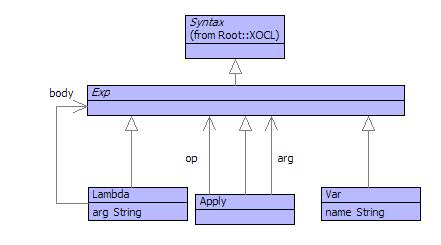
\includegraphics[width=12cm]{LanguageEngineering/SECD/Images/BasicCalculus}

\caption{Lambda Calculus\label{fig:Lambda-Calculus}}

\end{center}
\end{figure}


The lambda-calculus syntax is modelled in figure \ref{fig:Lambda-Calculus}.
The class Exp extends Syntax so that lambda expressions are self-evaluating.
The grammar is as follows:

\begin{lstlisting}
@Grammar
  Exp ::= Exp1 'end'.
  Exp1 ::= Lambda | a = Atom Composite^(a).
  Lambda ::= '\' a = Name '.' e = Exp1 { Lambda(a,e) }.
  Composite(a) ::= 
    b = Atom c = { Apply(a,b) } Composite^(c) 
  | b = Lambda { Apply(a,b) } | { a }.
  Atom ::= Var | Integer | '(' Exp1 ')'.
  Field ::= n = Name '=' e = Exp1 { Field(n,e) }.
  Var ::= n = Name { Var(n) }.
end 
\end{lstlisting}The definition of Composite provides an interesting feature: left
association. Applications are left associative in the lambda-calculus,
therefore the expression a b c is grouped as the application a b applied
to c, or equivalently (a b) c. The Composite rule is defined using
an argument a that accumulates the applications to the left.

%
\begin{figure}
\begin{center}

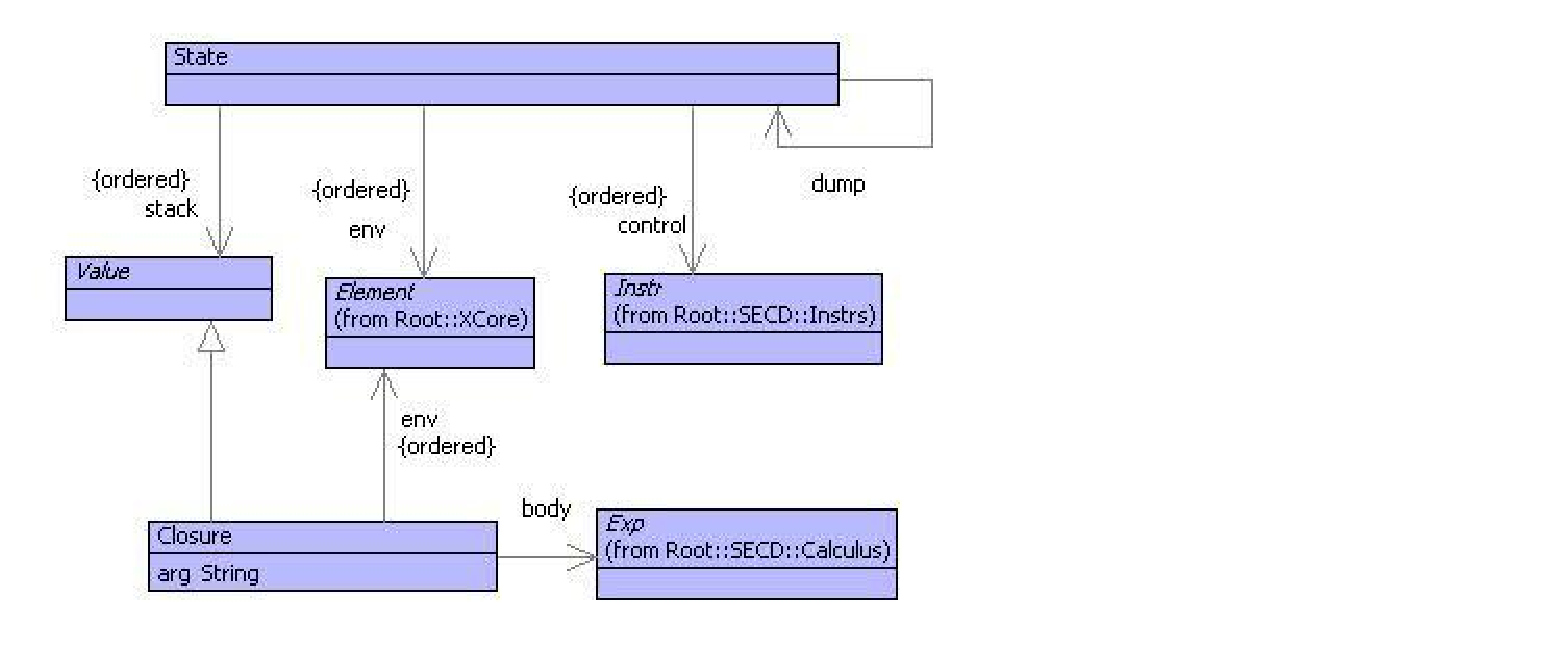
\includegraphics[width=12cm]{LanguageEngineering/SECD/Images/BasicMachine}

\caption{Machine States\label{fig:Machine-States}}

\end{center}
\end{figure}


Execution of lambda-calculus expressions can be performed by the SECD
machine (whose states are shown in figure \ref{fig:Machine-States}),
so-called because it has 4 components:

\begin{enumerate}
\item The \textit{stack} S that is used to hold intermediate results from
expressions.
\item The \textit{environment} E that is used to associate variable names
with values.
\item The \textit{control} C that is used to hold sequences of machine instructions.
\item The \textit{dump} D that is used to hold resumptions.
\end{enumerate}
%
\begin{figure}
\begin{center}

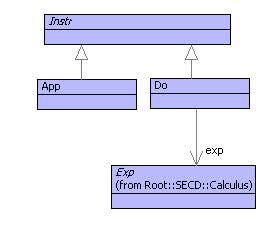
\includegraphics[width=12cm]{LanguageEngineering/SECD/Images/BasicInstrs}

\caption{Control Instructions\label{fig:Control-Instructions}}
\end{center}
\end{figure}


Execution of the machine is performed by case analysis on the instruction
at the head of the control. The instructions are shown in figure \ref{fig:Control-Instructions}.
Any expression is translated into an instruction using Do. the App
instruction is used to perform an application as shown below.

The best way to see what how the SECD machine works is to see it running.
The following trace shows the execution of an expression (\textbackslash{}v.
v v)(\textbackslash{}x.x). In order to make the output readable, the
following pretty-printers have been defined for the various classes:
States: (s,e,c,d); sequences: {[}x1,x2,x3]; pairs: h->t; App: @; Do:
ignored.

\begin{lstlisting}
(1) ([],[],[(\v.v v) (\x.x)],null)
(2) ([],[],[(\x.x),(\v.v v),@],null)
(3) ([<x,[],x>],[],[(\v.v v),@],null)
(4) ([<v,[],v v>,<x,[],x>],[],[@],null)
(5)   ([],[v-><x,[],x>],[v v],([],[],[],null))
(6)   ([],[v-><x,[],x>],[v,v,@],([],[],[],null))
(7)   ([<x,[],x>],[v-><x,[],x>],[v,@],([],[],[],null))
(8)   ([<x,[],x>,<x,[],x>],[v-><x,[],x>],[@],([],[],[],null))
(9)     ([],[x-><x,[],x>],[x],
          ([],[v-><x,[],x>],[],
            ([],[],[],null)))
(10)    ([<x,[],x>],[x-><x,[],x>],[],
          ([],[v-><x,[],x>],[],
            ([],[],[],null)))
(11)  ([<x,[],x>],[v-><x,[],x>],[],([],[],[],null))
(12)([<x,[],x>],[],[],null)
\end{lstlisting}The first thing to appreciate about the evaluation is roughly what
the expression is doing: the function \textbackslash{}v.v v is aplied
to the function \textbackslash{}x.x causing the function \textbackslash{}x.x
to be applied to itself producing the result \textbackslash{}x.x.
Now look at the trace and step through it to see how a machine evaluates
the expression. Each step in the trace is a new machine state produced
from the previous state by performing a transition. A transition looks
at the head of the control in the pre-state to determine the next
state.

Line (1) is the initial state. the expression is loaded onto the control.
Everything else is empty. Transition (1-2) performs the application
expression by unpacking it at the head of the control and adding an
@ instruction. Transition (2-3) evaluates the function \textbackslash{}x.x
to produce the closure at the head of the stack. Notice how the stack
is used to hold intermediate results; machine transitions consume
0 or more values at the head of the stack and produce 0 or 1 new values
at the head of the stack. Transition (3-4) evaluates the function
\textbackslash{}v. v v. Transition (4-5) performs the @ instruction
by setting up the evaluation of the body of the operator. The state
of the machine is saved in the dump so that the return value from
the application can be used. Notice how the envirnment in the new
state (5) contains a binding for the arg v. Transition (5-6) evaluates
the application v v. Transitions (6-9) evaluate the two references
to the variable v and then perform the application (again saving the
current state for return). Transition (9-10) evaluates the reference
to x and (10-11) returns a value since the control is exhausted. Transition
(11-12) perfoms the final return leaving the value of the original
expression at the head of the stack.

The rules of evaluation for the basic lambda-calculus are very simple.
They can be described using pattern matching and are defined in the
operation trans below that performs a single transition. A good understanding
of the rules of evaluation and their many variations is an excellent
basis for a deep understanding of how modelling can inform and enrich
programming.

\begin{lstlisting}
@Operation trans(state:State):State
  @Case state of
(1) State(s,e,Seq{Do(Var(n))|c},d) do
      State(Seq{e.lookup(n)|s},e,c,d)
    end
(2) State(s,e,Seq{Do(Apply(o,a))|c},d) do
      State(s,e,Seq{Do(a),Do(o)} + Seq{App()|c},d)
    end
(3) State(Seq{Closure(n,e1,b),a} + s,e2,Seq{App()|c},d) do
      State(Seq{},e1.bind(n,a),Seq{Do(b)},State(s,e2,c,d))
    end
(4) State(s,e,Seq{Do(Lambda(n,b))|c},d) do
      State(Seq{Closure(n,e,b)|s},e,c,d)
    end
(5) State(Seq{v},e1,Seq{},State(s,e2,c,d)) do
      State(Seq{v|s},e2,c,d)
    end
  end
end
\end{lstlisting}Transition (1) evaluates a variable by looking its name up in the
current environment and pushing the value on the stack. Transition
(2) unpacks an application at the head of the control. Transition
(3) performs an @ instruction at the head of the control. It expects
a closure above an argument at the head of the stack. The current
state is pushed onto the dump and a new state is created from the
closure body and environment. Transition (4) defines evaluation of
a function. Finally, transition (5) describes how a value is returned
from a completed function application (the body is exhausted).


\section{Extending the SECD Machine}

As it stands, the calculus and its execution by the SECD machine does
not look much like a standard programming language. Using just the
features you have seen, it is possible to encode virtually all standard
programming language concepts. Doing so is a bit like a cryptic crossword
- fiendishly difficult and spectacularly rewarding.

Rather than work with models of programs at the basic calculus level,
it is usual to add extensions. In fact, this is where the calculus
and its mechanical execution starts to be useful: if you have a requirement
to understand or design a new novel feature then see what you need
to do to add it to the calculus and SECD machine.

This section shows how the basic model can be extended by adding records,
integers and builtin operations such as +. A record is represented
as in {[}age=56, yearsService=10]. A tuple, or vector, is a record
where the fields have pre-determined names (usually represented as
numbers); for example a pair is {[}fst=1,snd=2] rather than (1,2).
This allows builtin operations to take tuples (represented as records)
as arguments: add{[}fst=1,snd=2] is the same as 1 + 2.

%
\begin{figure}
\begin{center}

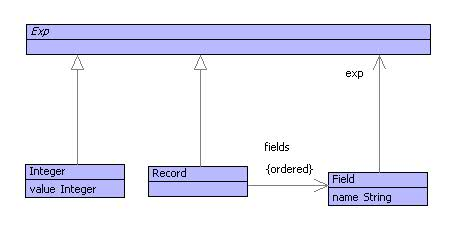
\includegraphics[width=12cm]{LanguageEngineering/SECD/Images/ExtendedCalculus}

\caption{Extended Syntax Model\label{fig:Extended-Syntax-Model}}

\end{center}
\end{figure}


The extensions to the syntax model are shown in figure \ref{fig:Extended-Syntax-Model}
and the grammar extension is shown below:

\begin{lstlisting}
Atom ::= Var | Record | Integer | '(' Exp1 ')'.
Record ::= '[' f = Field fs = (',' Field)* ']' { Record(Seq{f|fs}) }.
Field ::= n = Name '=' e = Exp1 { Field(n,e) }.
Integer ::= i = Int { Integer(i) }.
\end{lstlisting}The following shows an execution of the expression (\textbackslash{}x.\textbackslash{}y.add{[}fst=x,snd=y])
10 20. The builtin environment is shown as E. E contains a binding
for the name add to the builtin operation for +.

\begin{lstlisting}
([],E,[(\x.\y.add [fst=x,snd=y]) 10 20],null)
([],E,[20,(\x.\y.add [fst=x,snd=y]) 10,@],null)
([20],E,[(\x.\y.add [fst=x,snd=y]) 10,@],null)
([20],E,[10,(\x.\y.add [fst=x,snd=y]),@,@],null)
([10,20],E,[(\x.\y.add [fst=x,snd=y]),@,@],null)
([10,20],E,[\x.\y.add [fst=x,snd=y],@,@],null)
([<x,E,\y.add [fst=x,snd=y]>,10,20],E,[@,@],null)
  ([],E[x->10],[\y.add [fst=x,snd=y]],
    ([20],E,[@],null))
  ([<y,E[x->10],add [fst=x,snd=y]>],E[x->10],[],
    ([20],E,[@],null))
([<y,E[x->10],add [fst=x,snd=y]>,20],E,[@],null)
  ([],E[y->20,x->10],[add [fst=x,snd=y]],([],E,[],null))
  ([],E[y->20,x->10],[[fst=x,snd=y],add,@],([],E,[],null))
  ([],E[y->20,x->10],[x,y,{fst,snd},add,@],([],E,[],null))
  ([10],E[y->20,x->10],[y,{fst,snd},add,@],([],E,[],null))
  ([20,10],E[y->20,x->10],[{fst,snd},add,@],([],E,[],null))
  ([[fst=10,snd=20]],E[y->20,x->10],[add,@],([],E,[],null))
  ([!add,[fst=10,snd=20]],E[y->20,x->10],[@],([],E,[],null))
  ([30],E[y->20,x->10],[],([],E,[],null))
([30],E,[],null)
\end{lstlisting}
